\documentclass{beamer}

\usepackage{fontspec,xunicode,xltxtra}
\usepackage[french]{babel}
\usepackage{microtype}
\usepackage{default}	

\usepackage[]{hyperref}
\hypersetup{
	colorlinks=true}
\usetheme{simple}
\usepackage{graphicx}
\usepackage[utf8]{inputenc}
\usepackage[justification=centering]{caption}
\usepackage{subcaption}
\usepackage{listings}
\usepackage{pstricks}
\setmainfont{Merriweather Sans}
\setsansfont{Merriweather Sans}
\setmonofont{Fira Mono}
\captionsetup[subfigure]{labelformat=empty}
\captionsetup[figure]{labelformat=empty}
\setbeamertemplate{caption}{\raggedright\insertcaption\par}
\setbeamerfont{frametitle}{size=\LARGE}
\newfontfamily\DejaSans{DejaVu Sans}
\setbeamerfont{title}{family=\texttt,size=\huge}
\usepackage[scale=2]{ccicons}
\newfontfamily\unicodefun[Ligatures=TeX]{Symbola}

\title{Évolutions audio dans i-score}
\subtitle{à l'aide de la LibAudioStream}
\date{\today}
\author{Jean-Michaël Celerier}
\institute{LaBRI, Blue Yeti}

\newsavebox{\codebox}% For storing listings
\begin{document}
    
\maketitle
\begin{frame}
	\tableofcontents
\end{frame}
\section{Introduction}
\begin{frame}
    \frametitle{Problématique}    
    \Large
    \begin{itemize}
    	\item<1-> Audio fixé (type CD) \\ $\rightarrow$ \textbf{Cubase}, \textbf{Ardour}, \textbf{FastTracker}\dots
    	\item<2-> Audio libre et génératif \\  $\rightarrow$ \textbf{Max/MSP}, \textbf{PureData}.
    	\item<3-> Un peu d'interactivité \\ $\rightarrow$ \textbf{Ableton Live}, \textbf{Bitwig Studio}.~\\
    \end{itemize}    
\end{frame}

\begin{frame}
	\frametitle{Objectifs}    
	\Large
	\begin{itemize}
		\item<1-> Fonctionnement de séquenceur audio dans i-score, qui conserve les possibilités du formalisme.
		\item<2-> Support des effets, et graphes temporels d'effets.
		\item<3-> Précision d'écriture la plus élevée possible.
	\end{itemize}    
\end{frame}

\begin{frame}
	\frametitle{Méthode}    
	\Large
	\begin{itemize}
		\item<1-> Gestion de la \textbf{hiérarchie} et d'\textbf{audiographes} dans la LibAudioStream\cite{letzlibaudiostream}.
		\item<2-> Équivalence des structures temporelles de i-score dans la lib.
		\item<3-> Création de processus i-score correspondant aux fonctionnalités de la lib.
	\end{itemize}    
\end{frame}

\subsection{Processus audio}
\begin{frame}	
	\frametitle{Processus offerts}    
	\Large
	Rappel : \textbf{processus} : quelque chose qui s'exécute sur une durée. Par opposition à l'\textbf{état}, instantané.
	\begin{itemize}
		\item Lecture de fichier son (\textbf{Audio}).
		\item Chaîne d'effets audio (\textbf{Effects}).
		\item Processus audiographe (\textbf{Send}, \textbf{Return}).
		\item Processus de mixage (\textbf{Mix}).
	\end{itemize}    
\end{frame}

\section{Audiographes}
\subsection{Définitions}
\begin{frame}
	\frametitle{Audiographes...}    
	\Large
	\begin{itemize}
		\item On veut pouvoir réutiliser un même AudioStream à plusieurs endroits :  \\ $\rightarrow$ \textbf{Flowgraph} comme dans PureData, Max\dots
		\item Pour qu'un effet fonctionne, le flux à l'origine de l'effet doit l'être aussi.~\\
		La construction des AudioStream \textbf{impose un ordre}.
		\item Graphe de dépendances + tri topologique $=$ création des flux dans l'ordre.
	\end{itemize}    
\end{frame}

\subsection{Audiographes dans i-score}
\begin{frame}
	\frametitle{... dans i-score}    
	\Large
	
    On utilise comme unité de mixage la contrainte temporelle : 
    chaque contrainte se mixe dans son processus parent.
	
	\begin{figure}
		\centering
		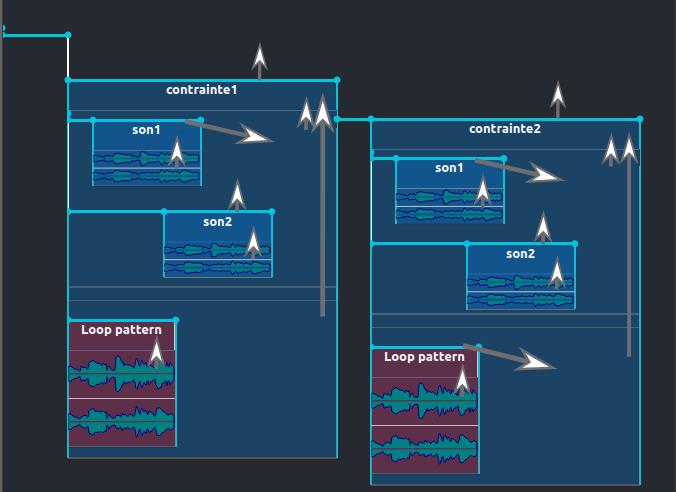
\includegraphics[width=0.6\textwidth]{images/mixage.png}
		\caption{Les objets se mixent en suivant les flèches}
	\end{figure}
\end{frame}

\begin{frame}
	\frametitle{Graphe de mixage}    
	\Large
	\begin{columns}
		\begin{column}{0.5\textwidth}
			\begin{figure}
				\centering
				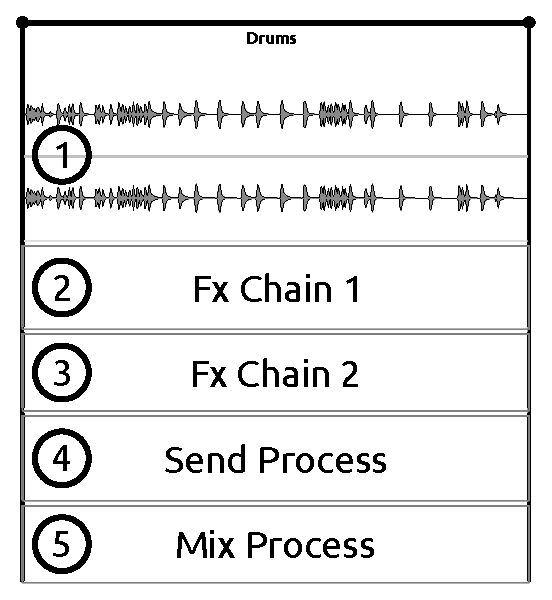
\includegraphics[width=\textwidth]{images/iscore1.eps}
				\caption{Une contrainte munie de 5 processus dans i-score}
			\end{figure}
		\end{column}
		\begin{column}{0.5\textwidth}
			\begin{figure}
				\centering
				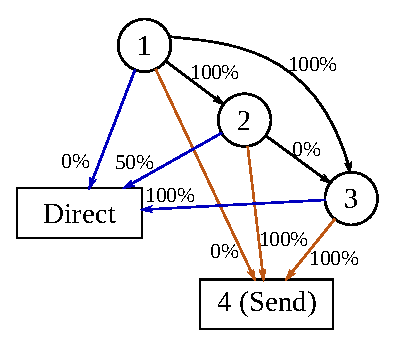
\includegraphics[width=\textwidth]{images/graph1.eps}
				\caption{La manière dont ces processus peuvent être traduits en graphe. 
					Le dosage est donné dans le \textbf{Mix Process}.}
			\end{figure}
		\end{column}
	\end{columns}
\end{frame}

\subsection{Graphes d'effets temporels}
\begin{frame}
	\frametitle{Audiographes}    
	\Large
	\begin{figure}
		\centering
		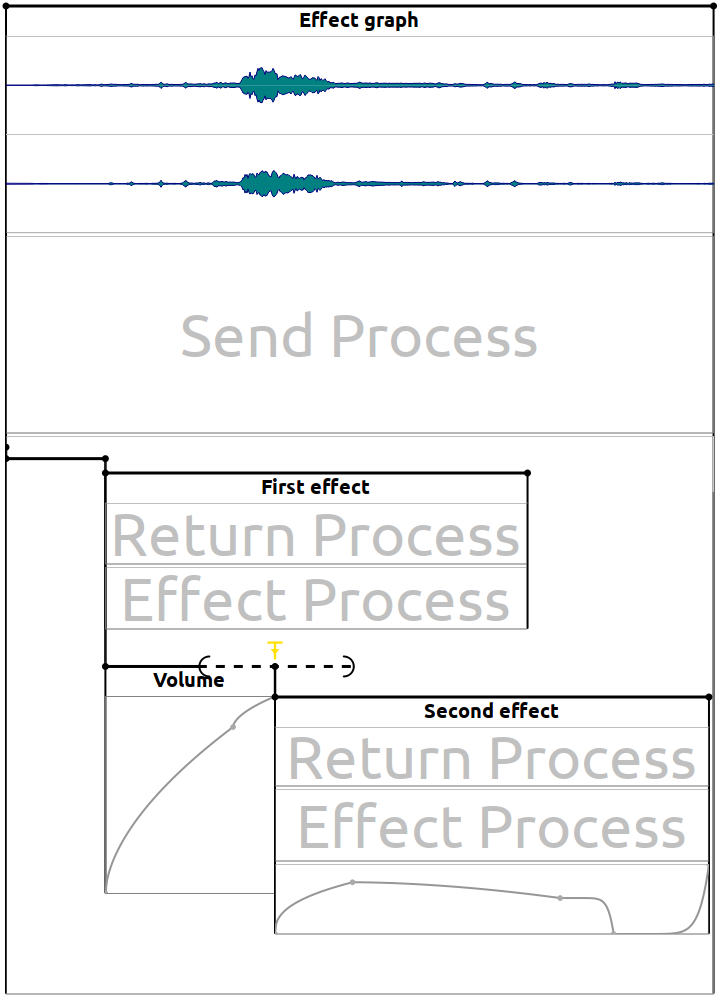
\includegraphics[width=0.4\textwidth]{images/ex3.png}
		\caption{Processus Send et Return pour partager un son entre plusieurs contraintes.}
	\end{figure}
\end{frame}

\section{Précision}
\begin{frame}
	\frametitle{Précision : cas des séquences}
	\Large
	
	\begin{columns}
		\begin{column}{0.5\textwidth}
			\begin{figure}
				\centering
				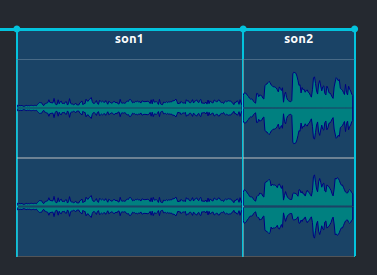
\includegraphics[width=\textwidth]{images/sequence.png}
				\caption{Le second son démarrera un échantillon après le dernier échantillon du premier son.}
			\end{figure}
		\end{column}
		\begin{column}{0.5\textwidth}
			\begin{figure}
				\centering
				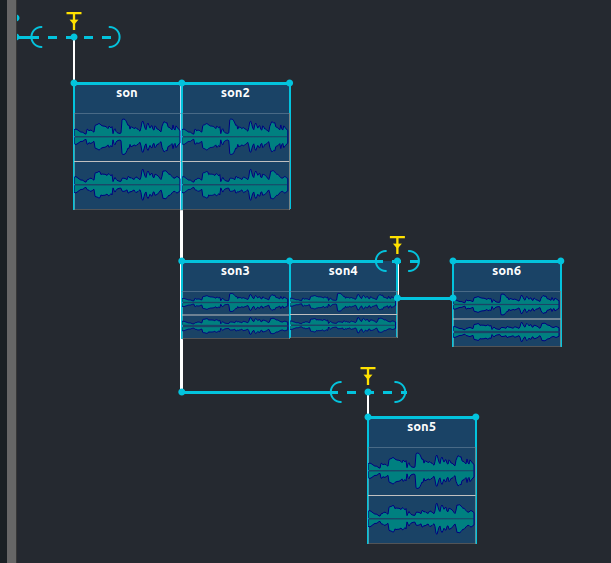
\includegraphics[width=\textwidth]{images/triggers.png}
				\caption{Lorsqu'un point d'interaction est déclenché, les nouvelles dates sont fixées jusqu'aux prochains points d'interaction}
			\end{figure}
		\end{column}
	\end{columns}
\end{frame}  

\begin{frame}
	\frametitle{Précision : cas des boucles}
	\Large
	
	\begin{columns}
		\begin{column}{0.5\textwidth}
			\begin{figure}
				\centering
				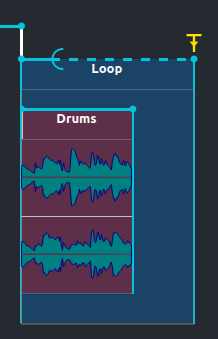
\includegraphics[width=0.62\textwidth]{images/loop.png}
				\caption{Chaque tour de boucle démarre un échantillon après le son précédent.}
			\end{figure}
		\end{column}
		\begin{column}{0.5\textwidth}
			\begin{figure}
				\centering
				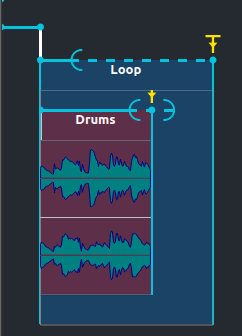
\includegraphics[width=0.7\textwidth]{images/loop2.png}
				\caption{Chaque tour de boucle démarre lors d'un déclenchement interactif.}
			\end{figure}
		\end{column}
	\end{columns}
\end{frame}  

\section{Introspection et effets}
\begin{frame}
	\frametitle{Introspection et effets}    
	\Large
	\begin{itemize}
		\item<1-> Actuellement : effets donnés en Faust.
		\item<2-> Chaque effet possède une liste de paramètres.
		\item<3-> Ces paramètres sont exposés dans l'arbre local d'i-score.
		\item<4-> Utilisables dans les automations, mappings, JS\dots
	\end{itemize}
	
	
	
\end{frame}

\begin{frame}
	\frametitle{Objectifs à venir} 
	\Large
	\begin{itemize}
		\item<1> Enregistrement, entrée audio.
		\item<2> Réutilisation en temps réel des enregistrements.
		\item<3> Meilleure intégration MIDI (piano roll ?).
		\item<4> Gestion des signatures temporelles.
		
	\end{itemize}
\end{frame}    

\begin{frame}
    \frametitle{Liens} 
    \Large
    \begin{itemize}
        \setlength\itemsep{1em}
        \item \textbf{Dépôt pour l'extension audio ({\unicodefun 🍎, 🐧})} :~\\
        \url{github.com/OSSIA/iscore-addon-audio}
        \item \textbf{Le logiciel} :~\\
         \url{i-score.org}
    \end{itemize}
        
    \centering
    \vspace{2em}
    \Large{Merci ! Questions ?}
    \vspace{2em}
    
    \tiny{Utilise le thème Beamer 'simple' de Facundo Muñoz; et les polices Fira, de Mozilla}
\end{frame}    

\begin{frame}
	\bibliographystyle{apalike}
	\bibliography{scrime2016}
\end{frame}
\end{document}
